\chapter{The project: MongoDB Performance}
\label{cha:3}
In this chapter the real core of this research, the project \textsc{MongoDB Performance}, is presented starting with the analysis  that we made before developing the software that consequently decreed the implementation choices.
Following there is an overview on the frameworks used and in the end the whole application is described in depth also showing screenshots of the user interface.

\section{Aim of the project and beginning idea}
\label{sec:1}
When benchmarking a product, the standard procedure is to compare it with its competitors, but in this case it took a while to the company to decide which kind of analysis could better fit the availability of time and money.
The beginning idea was in fact to build a software able to perform a stress test on different database technologies, and then to compare those tests and choose the one who could best support the requirements.
Technologies taken in account where MongoDB, Apache Cassandra and PostgreSQL with JSON datatype \footnote{https://www.postgresql.org/docs/9.6/static/datatype-json.html}, but after a meeting with the customer we decided to choose one technology for a specific test using as measurement parameters many benchmarks found on the web and the declared specifications, ease of use and configuration.
PostgreSQL was discarded almost immediately due to lower performance confirmed by third part benchmarks, so MongoDB became the first choice thanks to its simplicity and Cassandra was left as second choice in case Mongo couldn’t satisfy the requirements, even if it seemed to have better results on most of the benchmarks found on the Web. 
As mentioned, the customer gave us specific necessities:
\begin{itemize}
	\item The software counts many hundred thousand active users with thousands of records each one, so the database should be able to support several millions of total records.
	\item It works as a web application and needs to be responsive to give the user the best usage experience, consequently it should query results in no more than 2 seconds.
	\item It contains important billing information, so data cannot be lost.
	\item The web application is online 24/7 and it can be stopped only when releasing a new version. So even in the time slots with more expected traffic, any system crash must be prevented.
\end{itemize}
The final aim of the project so is not a benchmark between different DMBS, but a specific one performed on the chosen technology with the possibility to be eventually extended to other solutions.


\section{Implementation choices and architecture}
\label{sec:2}
It became clear that the beginning idea of a complete benchmark over the most used DBMS was impossible in term of time and money costs.
I decided to develop a modular application following the patterns of microservices. Due to this choice, the final result allows reusing a good part of the software  adding a new module for each eventual DMBS, using the existing code from the MongoDB module and adapting it to another database technology with the proper drivers provided by Java Spring.
In the end thanks to the satisfactory results obtained by MongoDB, there was no need to include other technologies in the benchmark.
The architecture, drew with \textit{Draw.io} \footnote{https://www.draw.io}, presents  both the implemented modules and the possible or discarded modules (dot-line) to give an overview of how a microservices production application should look
Due to time issues, we decide to not implemented all unnecessary modules like for example the \textit{Authentication Module}.
\begin{figure}
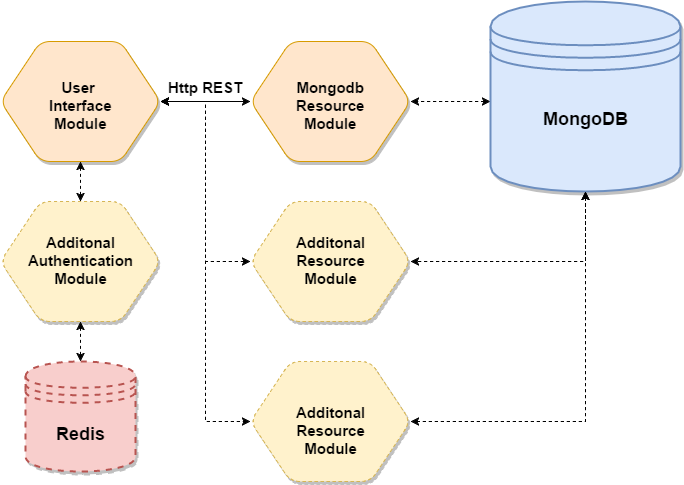
\includegraphics[scale=0.5]{app-architecture.png}
\centering
\caption{Representation of the architecture including possible future implementations}
\end{figure}



\section{Java Spring and AngularJS}
\label{sec:3}
\textsc{Spring} framework has become over the years one of the most popular Java frameworks for building  Enterprise applications, becoming an alternative (or replacement) for the more classical Enterprise Java Beans (EJB)  \footnote{https://en.wikipedia.org/wiki/Enterprise\_JavaBeans}. It introduced the concept of \textit{aspect-oriented} programming that is a programming paradigm that aims to increase modularity by allowing the separation of cross-cutting concerns. It’s composed by many modules, including Spring Security for authorization and authentication, Spring Web for customization of web applications using RESTful web services and Spring Data Access working with \textsc{JDBC} \footnote{http://www.oracle.com/technetwork/java/javase/jdbc/index.html} and object-relational mapping tools to support both relational and NoSQL databases. 
Spring can create standalone “runnable” production-grade applications with Spring Boot, including an embedded Tomcat, and opinionated \textit{POMs} \footnote{https://maven.apache.org/guides/introduction/introduction-to-the-pom.html} to simplify Maven configuration and production-ready features.
Those features, such as metrics, health check together with externalized configuration make it the definitive framework for Java Web applications among the java developer community and  it immediately became my unquestionable choice thanks to its affinity to micro-services model.
On the front-end side, AngularJS was the perfect choice thanks to its natural affinity with Spring and Twitter Bootstrap and its routing management system for dynamic loading dynamic content inside single-page applications. I’ve chosen version 1.6 instead of the new version AngularJS 2, that has a different and more complex implementation and usage based on TypeScript, and I’ve made a wide use of it especially in the User Interface Module that manages the launch and data plotting  of the stress-test.

\section{Microservices and modularity}
\label{sec:4}
The \textit{Micorservices Architecture} \footnote{http://microservices.io/patterns} is a modern type of architecture for servers-side enterprise applications. It is designed following specific patterns to support different clients including browsers (desktop or mobile) and native mobile applications. Part of the modules in a Microservices application might expose API to communicate via web services like REST calls, to exchange messages that return HTML/JSON/XML response.
This approach allows major modularity in the developing process of a project involving a team or more where each member (or each team) works only on an assigned module.
The application must be easy to understand in all of its single parts to sustain several deployments on different machines in order to satisfy scalability and availability requirements.
Different frameworks can be used separately on selected modules and functions of the software should not be replicated within the modules.
This type of architecture has many advantages:
\begin{itemize}
	\item Each microservice is a small and independent software, easy to understand and to debug, that in case of fault will not affect other modules \footnote{But its missing functionality could interrupt the application working process.}.
	\item Development is easy to scale, simply connecting a new independent module or machine. In this way each service can be developed and deployed independently.
	\item Eliminates any commitment to a technology stack, in fact if a service needs major changes  it can be rewritten with a new technology stack without interfering with the system.
\end{itemize}
Of course there are some disadvantages to deal if an application is developed following Microservices pattern, for example the additional complexity that a distributed system has rather than a monolithic system.
A good organization is necessary to manage testing and deployment phases  to keep a low operational complexity in production because the functionality of each single module does not guarantee the functionality of the entire system.
Another problem could be the network overhead generated by several distributed JVM that consume more memory and  network bandwidth than a single monolithic application.
In conclusion, this architecture is highly suggested in those use cases where a distributed system  includes several features (or services) and serves different typologies of clients \footnote{Different apps on different operative systems}, such as Netflix, Amazon and Ebay that switched from a monolithic architecture to microservices.
\begin{figure}[H]
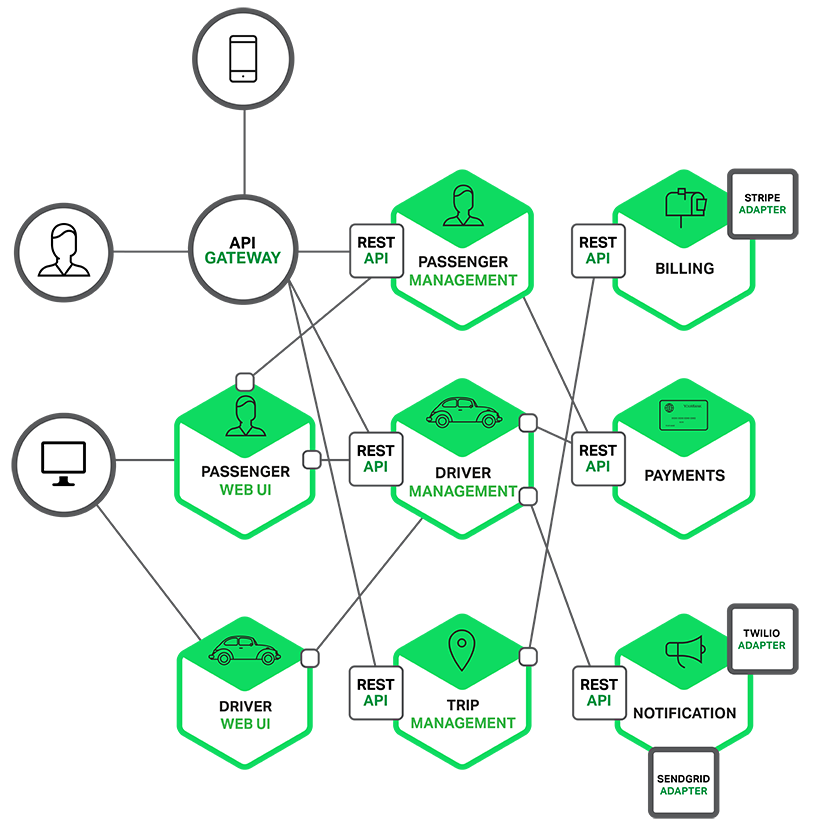
\includegraphics[scale=1.5]{microservices.png}
\centering
\caption{Example of architecture for an application like Uber.}
\end{figure}

\section{Final modules and possible implementations}
\label{sec:5}

\subsection{Architecture of the application}
The architecture was designed to be reusable and extensible following the theory of microservices. That’s why it was way more complex than the final result, with more modules each dedicated to provide a single functionality. The first design provided the following modules:
\begin{itemize}
	\item \textit{User Interface Module} : it has been kept in the final application and its functionality is related to serve the web resources that compose the front end of the application
	\item \textit{Authentication Module} : it was in beginning implemented and then removed because of possible usage complexity and also because of no real use during the main test. This module was connected to a \textsc{Redis} \footnote{https://redis.io} instance, that is a NoSQL database of key-value type with semi-persistence of the data through snapshots and was used to store the tokens to authenticate users of the application. Since there was need for only one user (me, as admin), the authentication service has been rewritten as angular module \textit{auth.js} for a single user inside the \textit{User Interface Module}. Anyway, it is still possible to add this module to the application for further usages in the future, as it is good practice to keep separated authentication from other features.
	\item \textit{MongoDB Resource Module} : is the main module that connects to MongoDB and its functionality is related to perform all the tasks needed for the stress test.
	\item \textit{Additional Resource Modules} : these modules are all the\textit{n} modules siblings of \textit{MongoDB Resource Module} that could be implemented to support different DBMS for the application. None of them have been actually realized and I decided to show only two in the schema as reminder for the possibilities taken into account at the beginning of the project but discarded for the motivations explained in chapter 2, Apache Cassandra and PostgreSQL with JSON datatype
\end{itemize}

\subsection{User Interface module}
The \textit{UI Module} is a standalone Java Spring application that serves all the static content, libraries and web pages, to a local host server where the user can login and start using the application. There is a single web page where the content is dynamically loaded using AngularJS routing through modules.
The Login Page does not allow a non-authenticated user to use the application, and its functionality is provided by \textit{auth.js} angular module. After correct login, it is possible to start navigating other sections.
\begin{figure}[H]
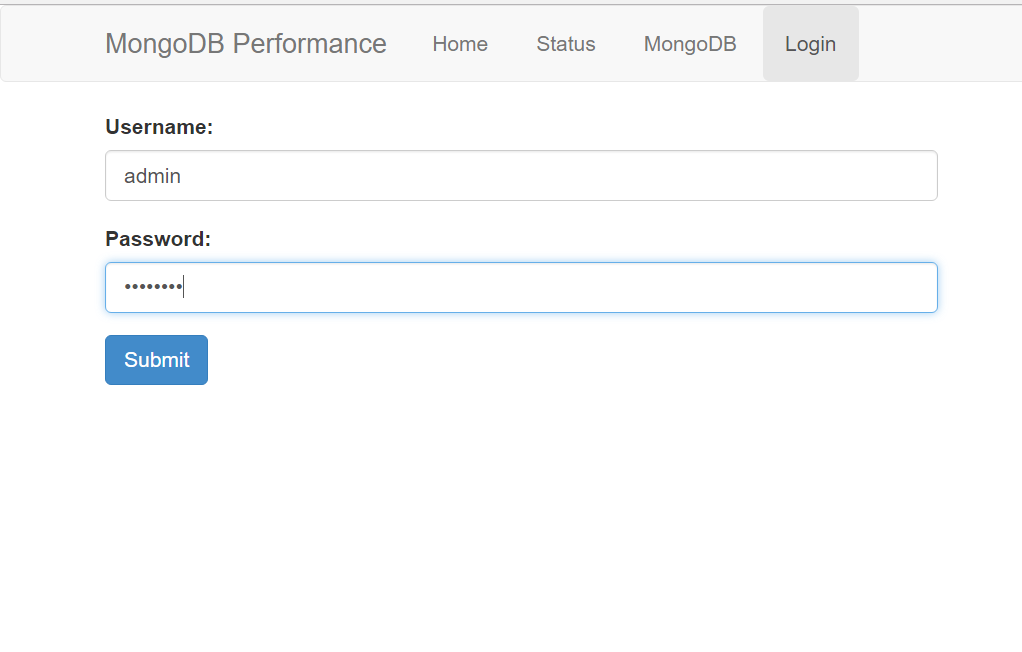
\includegraphics[scale=0.5]{login.png}
\centering
\caption{The Login page.}
\end{figure}
The \textit{Home Page} simply introduce the user to the application with a welcoming message.
The \textit{Status Page} is  a page that launches a REST \footnote{https://en.wikipedia.org/wiki/Representational\_state\_transfer} call to all modules that are supposed to be in the application to check and monitor their status, then it prompts the result on screen. It makes easy to discover if a module, even running on another machine, is not answering allowing the user to quickly resolve the problem.
\begin{figure}[H]
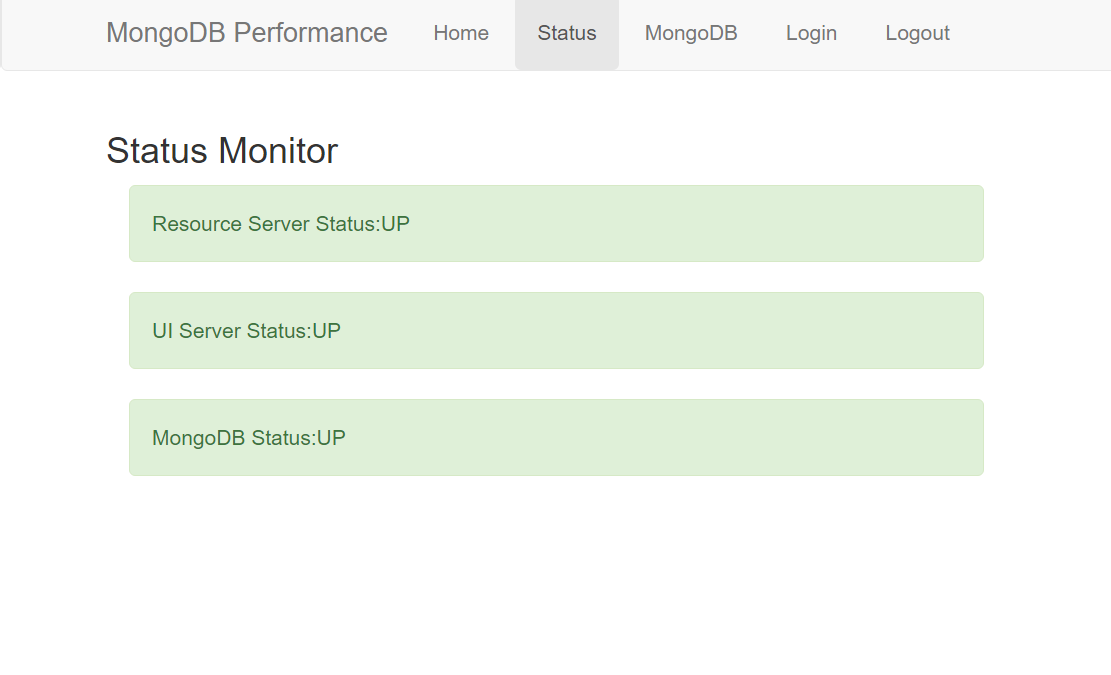
\includegraphics[scale=0.5]{status.png}
\centering
\caption{The Status page.}
\end{figure}
The\textit{MongoDB Page} is the most important of this module and  it is the page where the user can set up the configuration for a new test.
It is possible to choose:
\begin{itemize}
	\item The\textit{ number of entries} or inserts that has to be performed during the whole test
	\item The \textit{number of threads}, each one simulates a new client connecting to the MongoDB node. It is important to specify that the number of entries of each thread will be the total number of entries / the total number of threads. There is no real limit to the number that can be set, but a normal notebook will begin to suffer with more than 8 threads as the Java Virtual Machine is pretty expensive on the CPU and on the RAM. We will see further the specifications of the machines used during the experiment and how many threads have been used for the test.
	\item The \textit{type of test}, using only \textsc{put} statements (only inserts), only \textsc{get} statements (only gets, never used in practice) or \textsc{put/get} statements (one insert and then one get for each entry).
	\item The \textit{IP address} of the machine or computer running an instance of the Resource Module, to choose where start a test or to monitor an already running test on a specific machine.
\end{itemize}
\begin{figure}[H]
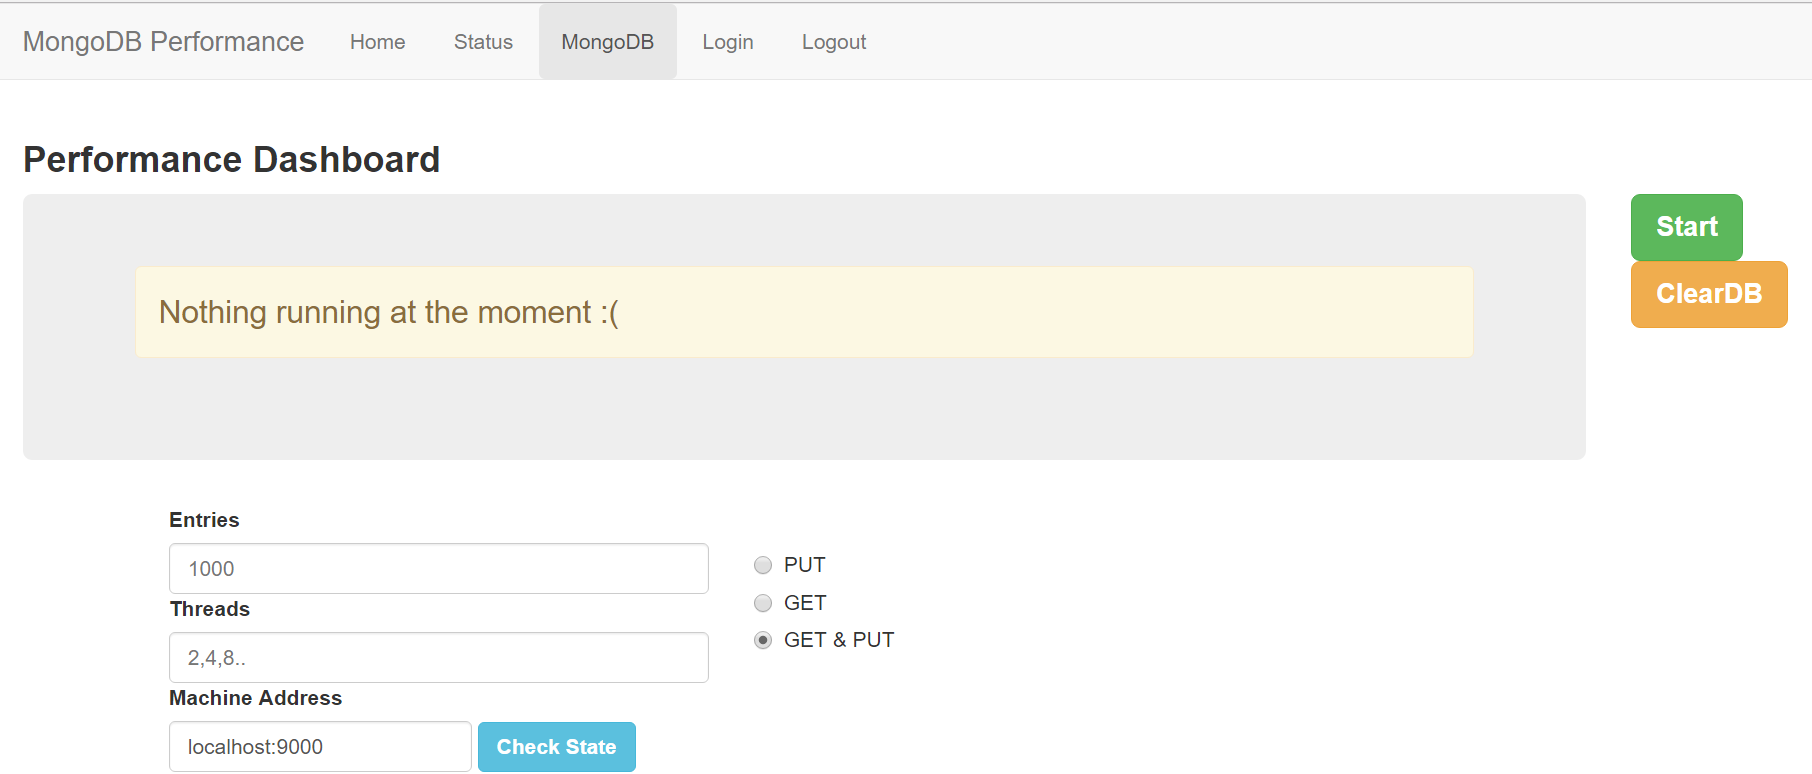
\includegraphics[scale=0.3]{test-off.png}
\centering
\caption{The MongoDB page.}
\end{figure}
It is  possible to drop all the records in the database to clean it up before a new test using the button “ClearDB”. When everything is set up, or using default values, it is possible to “Launch” the test and open  new view that shows any possible information about the running test. It is important to specify that in absence of a responding Resource Module, the test won’t start because all the metrics are calculated in that module and fetched through REST calls.
If everything is correctly set up, the test will start and all metrics calculated on Mongo are fetched and showed in the top table.
\begin{figure}[H]
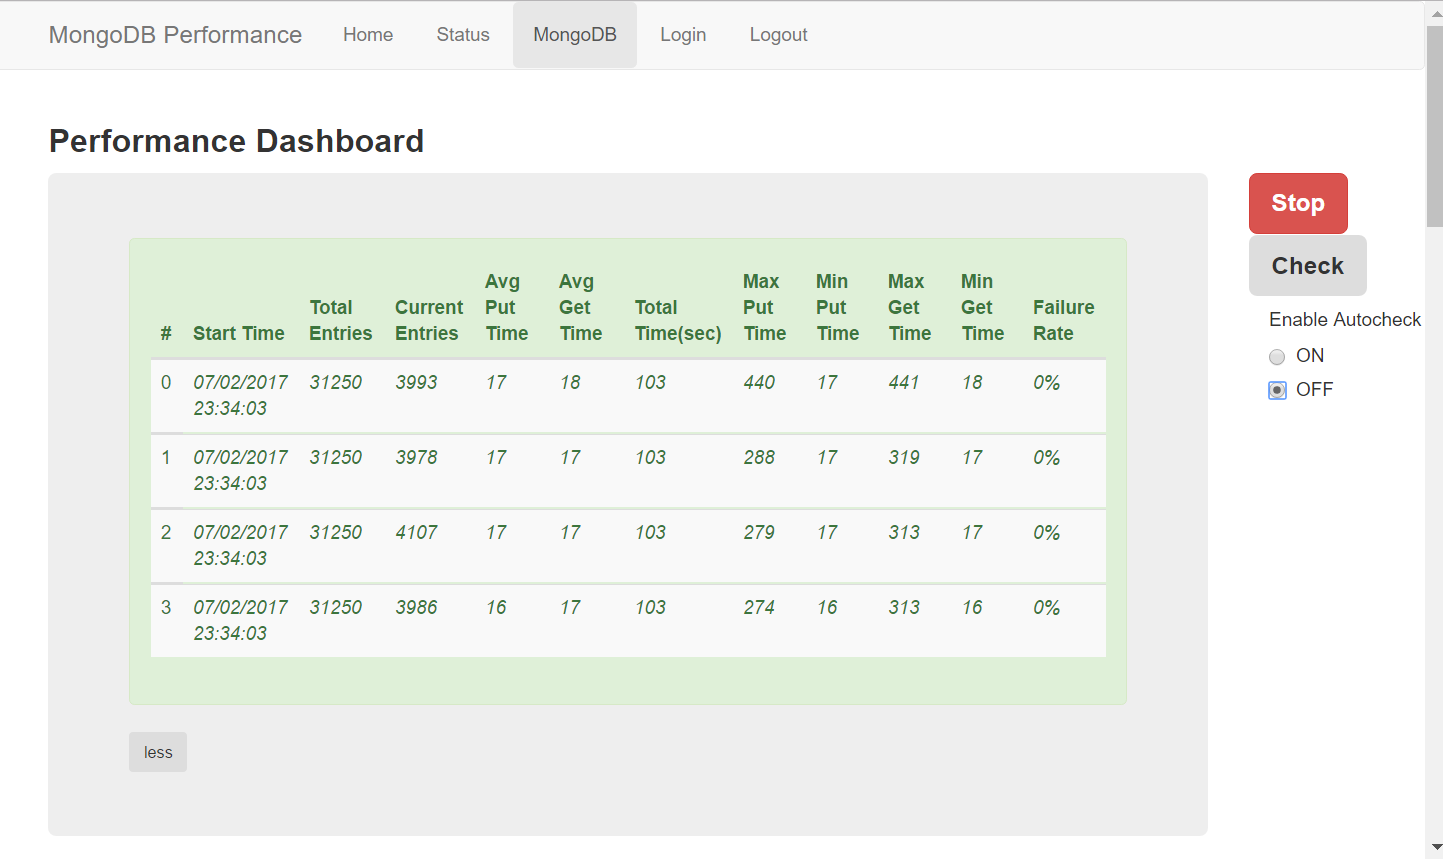
\includegraphics[scale=0.4]{metriche.png}
\centering
\caption{Table of the metrics.}
\end{figure}
It is possible to plot  the most interesting metrics in real time with “AutoDraw”  , but this option is disabled by default due to the heavy cost in terms of memory for the computer. It is anyway possible to plot metrics at the end of the test with “Draw” because all data are saved in variables until the test is not stopped. All graphs and tables that will be presented in the tests have been plotted by the application and saved at the end of each test.
\begin{figure}[H]
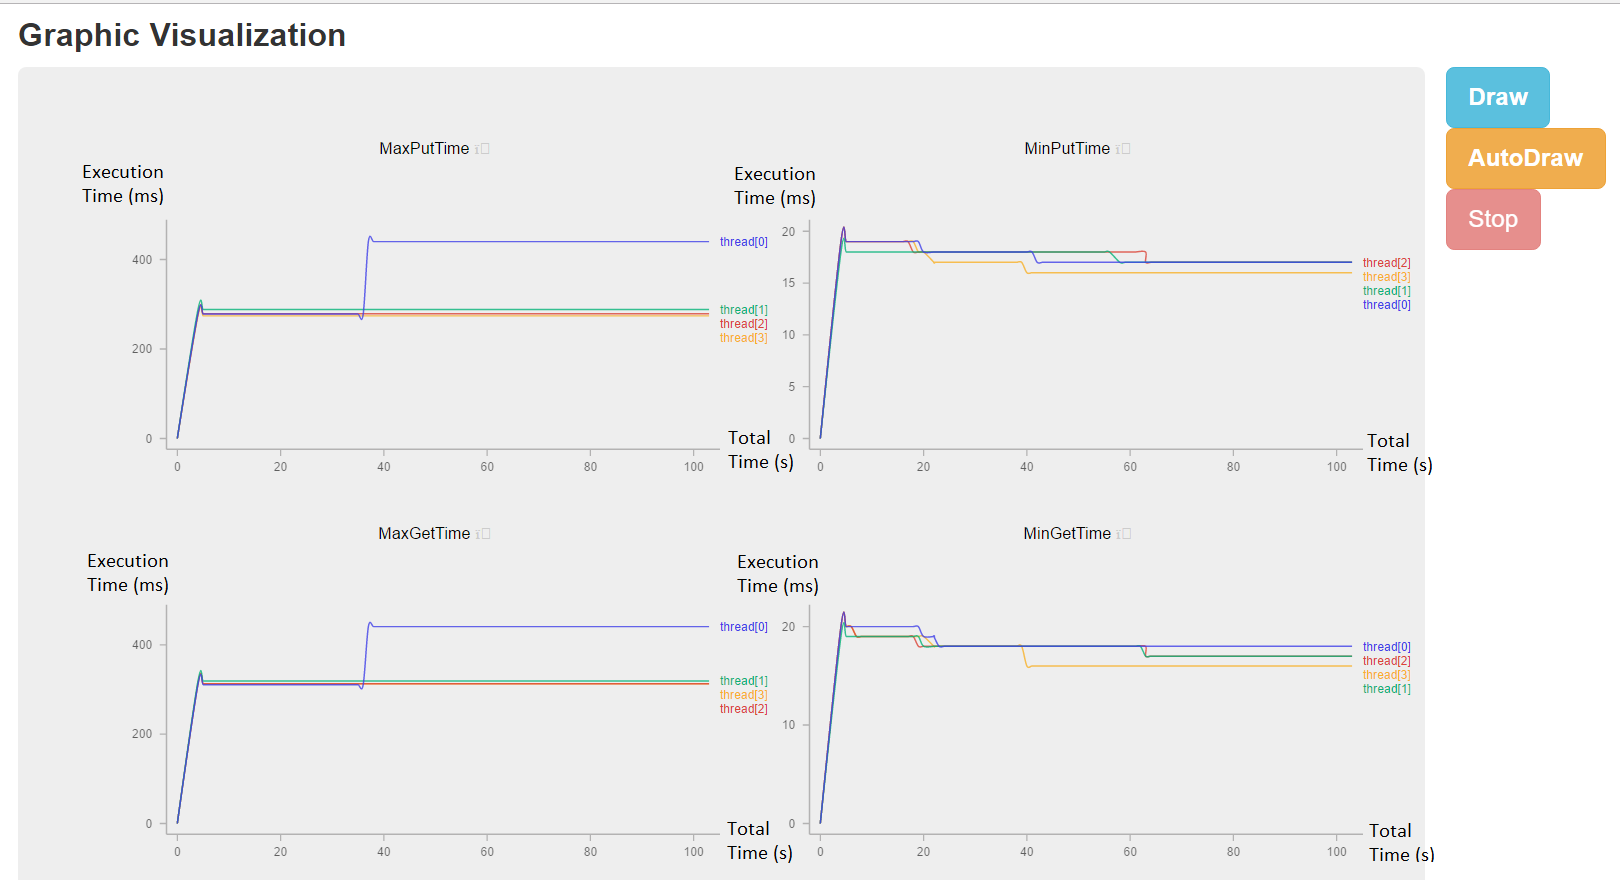
\includegraphics[scale=0.6]{grafici_corretti.png}
\centering
\caption{Graphics of Min/Max Put/Get times.}
\end{figure}
\begin{figure}[H]
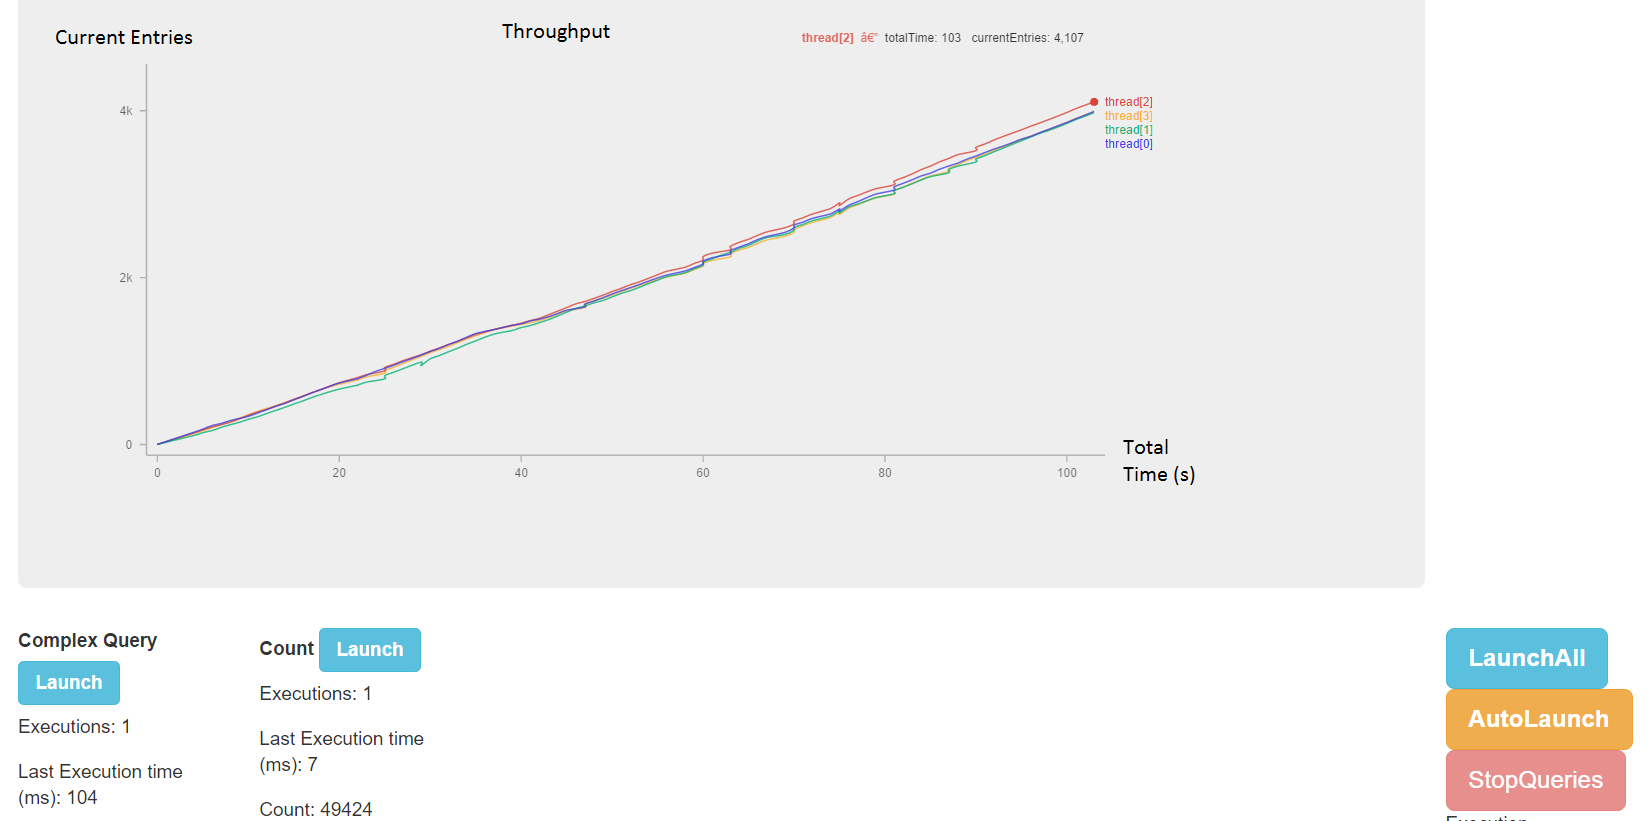
\includegraphics[scale=0.6]{queries_corrette.png}
\centering
\caption{Graphic of Throughput and query commands.}
\end{figure}
At the bottom of the page there are two buttons that can launch specific queries:
\begin{itemize}
	\item \textit{countAll( )} - Query that returns all the current records in the database. The main reason for this was to double check the insertions and see if they matched the values printed in the metrics table.
	\item \textit{complexQuery( )} - Query with the purpose to stress the  process of insert and get of the entries, it was used in specific tests with heavy workload and its times of execution where saved and then plotted in a secondary moment. When launched in “Auto” it runs every 10 seconds and updates an array containing all the execution times that will be plotted.\footnote{See section 4.4}
\end{itemize}



\subsection{MongoDB Resource module}
This is the core module of the application. All endpoints for the REST calls from the UI Module are defined and connected to a specific function in this module. It is not necessary to have an UI Module to run a test since it is possible to launch the standalone .jar of the Resource Module from command line and setup a test following the options printed on screen. It is possible to print some metrics on the console, but this functionality has never been used during the benchmark due to the necessity of plotting data on the UI.
\begin{figure}[H]
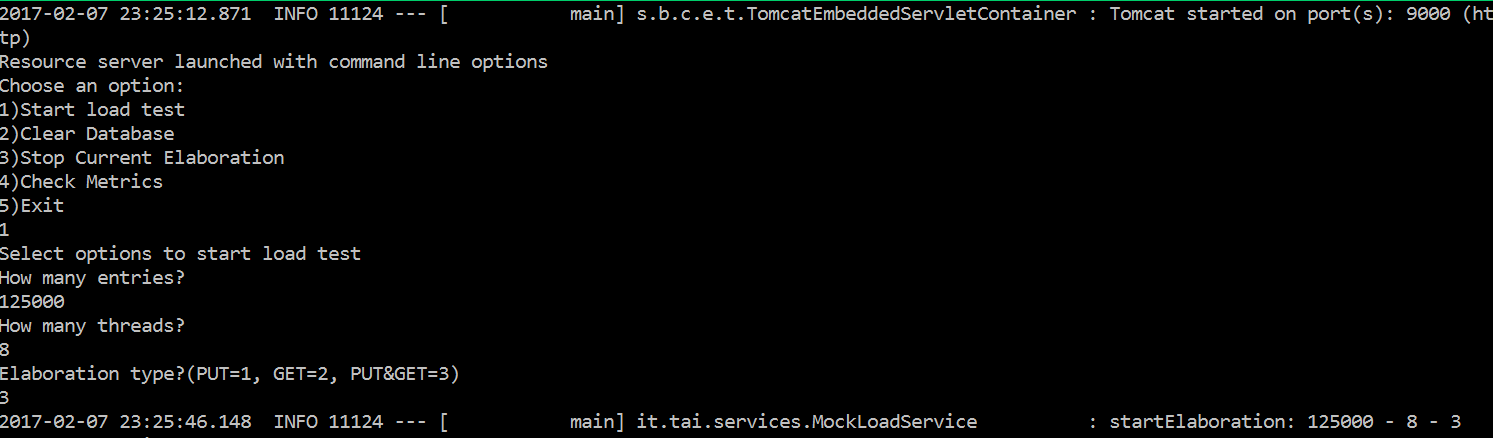
\includegraphics[scale=0.4]{command-line.png}
\centering
\caption{The Resource Module in the Linux shell.}
\end{figure}
It is possible to connect the UI Module to different instances of the Resource Modules even running of different machines to fetch all possible data, and this is how the tests have been conducted.
In this module is also defined the structure of \textit{Fattura.java}, the type of document used for the tests, and the repository that connects to the MongoDB collection Test where the data are stored. The core class of the module is \textit{MockLoadService.java} where resides the algorithm that process the benchmark and where all the metrics are calculated and saved.
The algorithm takes as parameters the number of entries, the type of test and most important the number of threads; then for each thread it replicates the process simulating a new client connection on the database.
